\chapter{Android & Wi-Fi direct}

Android è un sistema operativo per dispositivi mobili sviluppato da Google, basato su kernel Linux.
La sua progettazione è principalmente per smartphone e tablet, ma possiede anche interfacce utente specializzate per televisori (Android TV), automobili (Android  Auto), orologi da polso (Android Wear), occhiali (Google Glass) ecc… .
Essendo basato su kernel Linux possiede una licenza (Licenza Apache) che consente di modificare e distribuire liberamente il codice sorgente. 
Inoltre, tutte le applicazioni sono scritte soprattutto in linguaggio di programmazione Java.
Ogni release del sistema possiede un nome simbolico ed è rigorosamente dato seguendo l'ordine alfabetico, ed inoltre ogni nome corrisponde ad una golosità presente nel mondo, qua di seguito la lista delle varie versioni: la 1.5 venne chiamata Cupcake, la 1.6 Donut, la 2.1 Eclair, la 2.2 Froyo, la 2.3 Gingerbread, la 3.0 Honeycomb, la 4.0 Ice Cream Sandwich, la 4.1 Jelly Bean, la 4.4 Kit Kat. 
Attualmente l’ultima versione del sistema operativo è la 5.0, chiamata Lollipop.


\section{API}

\subsection{Architettura Android}

L'architettura di Android si suddivide in vari livelli (o layer), ognuno dei quali offre un servizio a quello superiore.
Vediamoli nel dettaglio:

\begin{center}
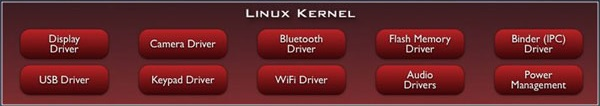
\includegraphics[width=1\textwidth]{imgs/Linux Kernel.jpg}
\captionof{figure}{Livello più basso dell'architettura Android}\label{linux_kernel_img}%
\end{center}

Nella figura \ref{linux_kernel_img} viene rappresentato il livello più basso di tale architettura, che contiene il kernel di Linux.
Inoltre, comprende anche vari driver per la gestione delle diverse periferiche: dallo schermo alla tastiera, dalla scheda di rete Wi-Fi all'alimentazione.

\begin{center}
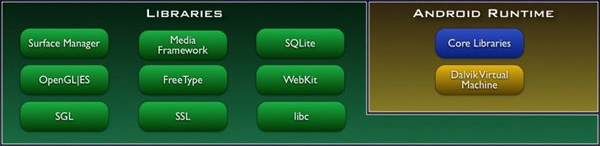
\includegraphics[width=1\textwidth]{imgs/Librerie.jpg}
\captionof{figure}{Tale livello rappresenta il cuore di Android}\label{librerie_img}%
\end{center}

Salendo invece al terzo livello, troviamo tutte le Librerie native che sono state svillupate nel linguaggio C/C++ figura \ref{librerie_img}.
Tutte insieme tali librerie rappresentano il cuore di Android, qui di seguito alcuni componenti delle librerie nello specifico: Surface Manager, che gestisce la componente grafica
Media Framework, implicata nella gestione dei codec audio e video
La libreria SSL che gestisce il Secure Socket Layer.

\begin{center}
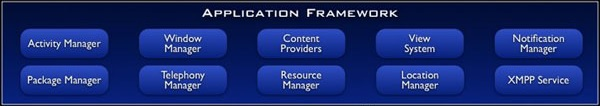
\includegraphics[width=1\textwidth]{imgs/Applicazioni_Framework.jpg}
\captionof{figure}{Livello composto da una serie di componenti API}\label{applicazioni_framework_img}%
\end{center}

Salendo ancora al quarto livello troviamo l'Application Framework figura \ref{applicazioni_framework_img}, formato da un insieme di API che svolgono specifici compiti:
Activity Manager, fondamentale in quanto è responsabile dell'interazione tra applicazione e utente.
Window Manager per la gestione delle finestre delle varie applicazioni.
Package Manager responsabile della gestione del ciclo di vita delle applicazioni.

\begin{center}
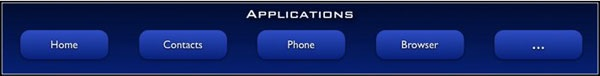
\includegraphics[width=1\textwidth]{imgs/Applicazioni.jpg}
\captionof{figure}{Ultimo livello che racchiude le applicazioni vere e proprie}\label{applicazioni_img}%
\end{center}

Arrivati all'ultimo livello, troviamo le Applicazioni vere e proprie che utilizzano i livelli sottostanti per essere eseguite figura \ref{applicazioni_img}.
Tra le tante applicazioni possiamo citare, calendario, rubrica, orologio.

\subsection{Ciclo di vita di un Applicazione (Activity)}

Nella sezione precedente abbiamo concluso parlando dell'ultimo livello, cioè quello che comprende le Applicazioni vere e proprie, un applicazione
è un software che viene eseguito e gestito dal sistema operativo Android, che possiede un proprio ciclo di vita.


\begin{center}
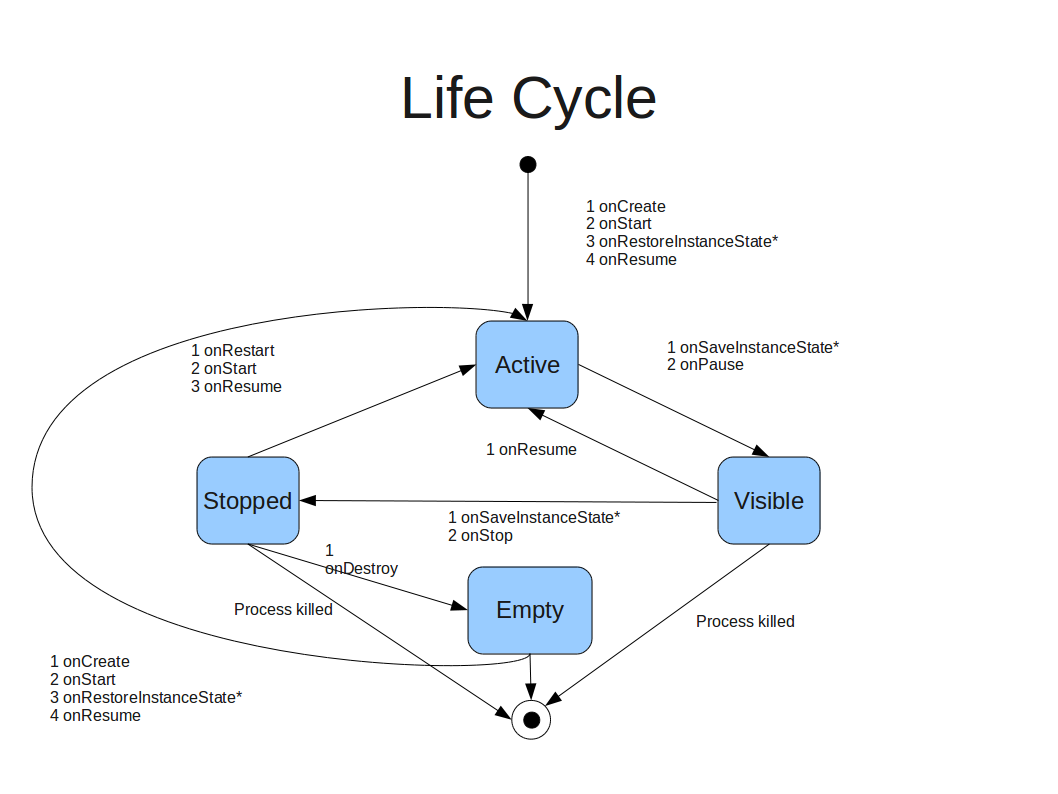
\includegraphics[width=1\textwidth]{imgs/ActivityLifeCycle.jpg}
\captionof{figure}{Rappresentazione ciclo di vita di un Activity}\label{activity_cycle_img}%
\end{center}

Come possiamo notare nella figura \ref{activity_cycle_img}, un ciclo di vita non è altro che una serie di stati attraverso i quali l'Activity passa.
I passaggi tra i diversi stati vengono notificati tramite una callback (metodo) invocata dal sistema.

Quando un activity viene mandata in esecuzione, vengono necessariamente invocati 3 metodi:
onCreate(): l'activity viene creata, e il programmatore dovrà definire le configurazione di base e il layout.

onStart(): l'activity diventa visibile, ed è il momento in cui i servizi e le funzionalità vengono attivate per fornire informazioni all'utente.

onResume(): l'activity diventa la destinazione di tutti gli input dell'utente.

Nel caso in cui l'Utente riceva una chiamata o più semplicemente apra un applicazione diversa, il sistema Android mette a risposo l'applicazione che stava usando in quel momento.
E anche per questa operazione verranno invocati 3 metodi:

onPause(): avverte che l'utente ha smesso di interagire con l'activity.

onStop(): indica la fine della visibilità dell'Activity.

onDestroy(): indica che l'Activity è stata terminata.

\section{Sketch codice}

\subsection{Wi-Fi Direct in Android}

Il Wi-Fi Direct chiamato anche Wi-Fi Peer to Peer (P2P) è disponibile sui dispositivi Android che posseggono la versione 4.0 (API 14), nonchè l'adeguato hardware.
Con tale tecnologia è possibile collegarsi e comunicare via Wi-Fi con un altro dispositivo, senza bisogno di un Access Point (AP) intermediario.

Tale tecnologia è basata su 2 parti fondamentali:

-Metodi, con la quale è possibile compiere le fasi di discover,request e connect verso i peer che sono indicati nella classe WifiP2PManager.

-Listener (oggetti), che si occupano di notificare il Successo o il Fallimento delle chiamate dei metodi contenuti nella classe WifiP2pManager.

-Intenti, che si occupano di notificare eventi specifici rilevati dal Wi-Fi P2P framework, per esempio una perdita di connessione o la scoperta di un nuovo peer.

Nella programmazione questi 3 metodi vengono usati spesso.
Un esempio pratico è l'uso di "WifiP2pManager.ActionListener" per chiamare il metodo discoverPeers(), se il metodo verrà eseguito correttamente verremo notificati dai metodi ActionListener.onSuccess() e ActionListener.onFailure().
Inoltre sarà anche trasmesso un intento chiamato WIFI P2P PEERS CHANGED ACTION nel caso in cui il metodo discoverPeers() rilevi modifiche tra la lista dei peer disponibili.

Per entrare ancora più nel dettaglio ecco una lista dei metodi, listener e intent contenuti nella classe WifiP2pManager:

\begin{center}
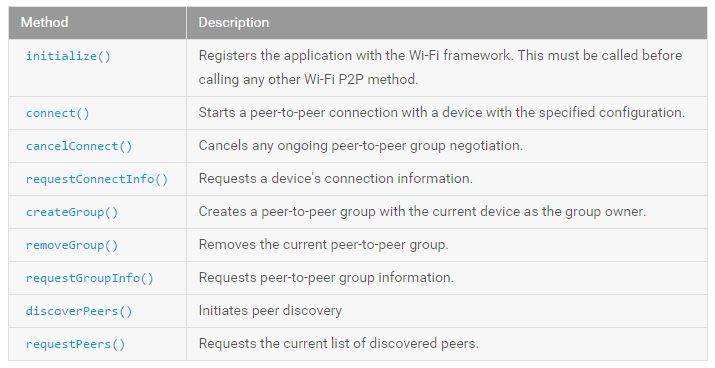
\includegraphics[width=1\textwidth]{imgs/p2pmethods.jpg}
\captionof{figure}{Lista dei Metodi persenti nella classe WifiP2pManager}\label{p2pmethods_img}%
\end{center}

\begin{center}
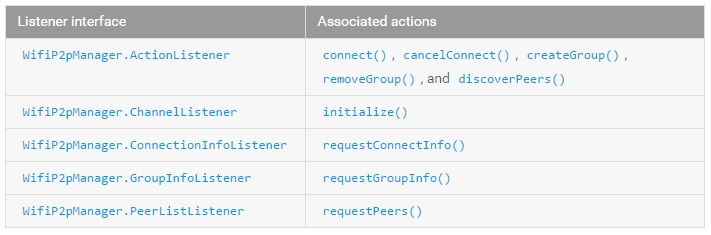
\includegraphics[width=1\textwidth]{imgs/p2plistener.jpg}
\captionof{figure}{Lista dei Listener persenti nella classe WifiP2pManager}\label{p2plistener_img}%
\end{center}

\begin{center}
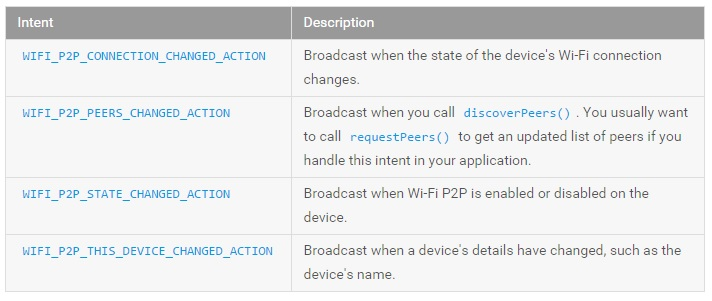
\includegraphics[width=1\textwidth]{imgs/p2pintents.jpg}
\captionof{figure}{Lista dei Intents persenti nella classe WifiP2pManager}\label{p2pintents_img}%
\end{center}

\subsection{Wi-Fi Direct in Pratica}

\subsubsection{Creazione classe BroadcastReceiver}

La creazione di una classe BroadcastReceiver è la base per lo sviluppo di un applicazione che vuole sfruttare il Wi-Fi Direct, in quanto permette di rispondere ad eventi (Intents) ricevuti di nostro interesse.
Ci sono 2 step base da seguire per la creazione di questa classe che permette di captare gli Intent Wi-Fi P2P e sono i seguenti:

1- Creazione di una classe che estenda la BroadcastReceiver.

2- Nella classe BroadcastReceiver eseguire la verifica degli Intent di nostro interesse all'interno del metodo       onReceive().
   Per esempio, se il BroadcastReceiver riceve un intento WIFI P2P PEERS CHANGED ACTION, si potrà chiamare il        metodo requestPeers() per avere una lista dei Peer trovati al momento.

   

\begin{center}
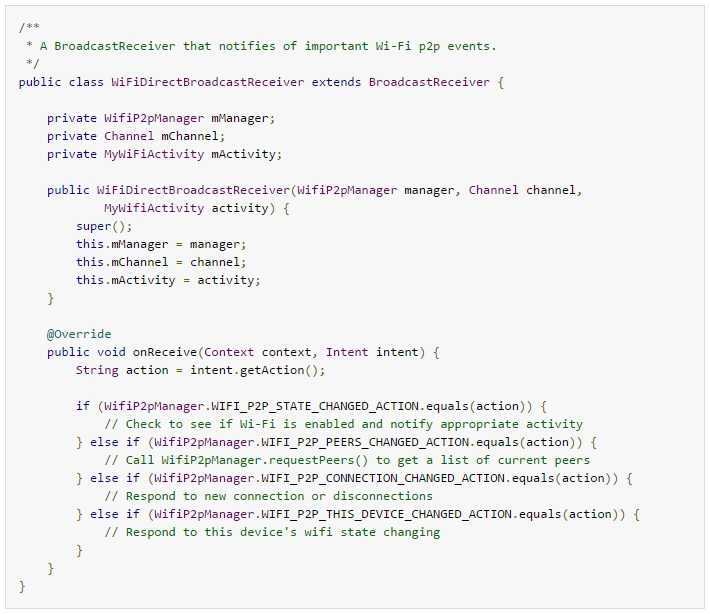
\includegraphics[width=0.9\textwidth]{imgs/broadcastreceiver.jpg}
\captionof{figure}{Rappresentazione classe BroadcastReceiver}\label{broadcastreceiver_img}%
\end{center}

\subsubsection{Creazione Applicazione Wi-Fi P2P}

Una volta creata la classe BroadcastReceiver possiamo procedere con lo sviluppo dell'applicazione vera e propria, di seguito seguiranno gli step passo passo.

1- Per prima cosa dobbiamo richiedere i permessi per usare l'hardware relativo al Wi-Fi, e per fare questo basta inserire il seguente codice all'interno di AndroidManifest:


\begin{center}
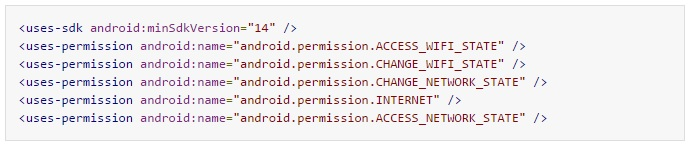
\includegraphics[width=1\textwidth]{imgs/manifest.jpg}
\captionof{figure}{Richiesta permessi di accesso a hardware Wi-Fi}\label{manifest_img}%
\end{center}

2- Eseguire un controllo sullo stato del Wi-Fi P2P ( acceso/spento, supportato o non supportato ): 
   
\begin{center}
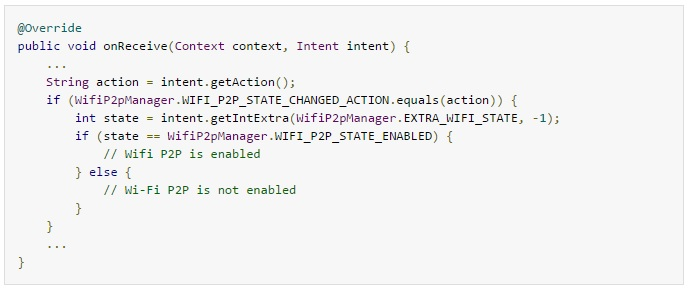
\includegraphics[width=1\textwidth]{imgs/check_wifi_avaiable.jpg}
\captionof{figure}{Controllo dello stato e del supporto del Wi-Fi P2P}\label{check_wifi_avaiable_img}%
\end{center}

3- All'interno del metodo onCreate(), bisogna creare un istanza WifiP2pManager e registrare la propria applicazione contenente il Wi-Fi P2P framework mediante il metodo initialize().
Tale metodo ritorna un WifiP2pManager.Channel (oggetto), con il quale sarà possibile connettersi al Wi-Fi P2P framework:

\begin{center}
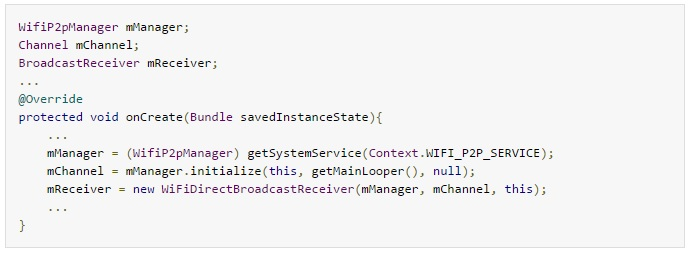
\includegraphics[width=1\textwidth]{imgs/onCreate.jpg}
\captionof{figure}{Metodo di connessione al framework}\label{onCreate_img}%
\end{center}

4- Creare un filtro di intenti, e aggiungere all'interno gli stessi intent contenuti nel BroadcastReceiver:

\begin{center}
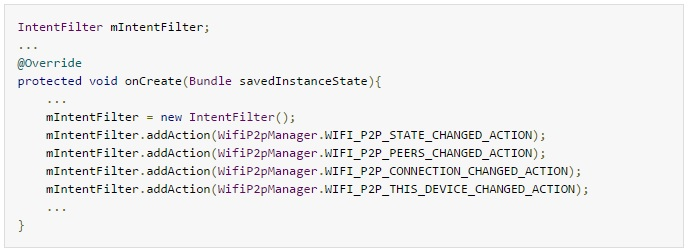
\includegraphics[width=1\textwidth]{imgs/intent_filter.jpg}
\captionof{figure}{Dichiarazione dei filtri per Intent}\label{intent_filter_img}%
\end{center}

5- Registrare il nostro BroadcastReceiver all'interno del metodo onResume() della nostra activity e cancellarlo dal metodo onPause():

\begin{center}
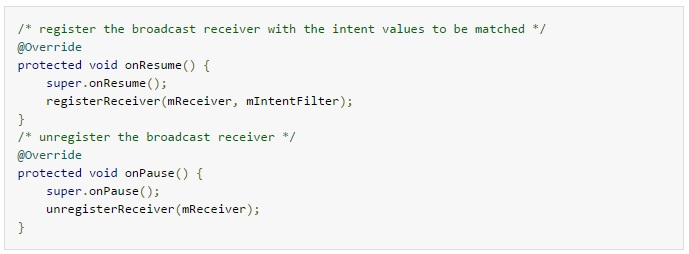
\includegraphics[width=1\textwidth]{imgs/register_receiver.jpg}
\captionof{figure}{Registrazione e cancellazione del BroadcastReceiver dai due metodi}\label{register_receiver_img}%
\end{center}

Una volta completati questi step, la tua applicazione sarà pronta per ricevere Wi-Fi P2P Intents ed effettuare chiamate dei metodi Wi-Fi P2P.

\subsubsection{Ricerca dei Peers (Utenti)}

Per ricevere la lista dei Peers disponibili alla connessione, bisogna effettuare una chiamata al metodo discoverPeers().
La chiamata di questo metodo funziona in modo asincrono, e il successo o fallimento di tale chiamata viene notificato dai metodi onSuccess() e onFailure() se è stato precedentemente creato un WifiP2pManager.ActionListener, da notare bene che tali metodi forniscono solo informazioni di successo o fallimento e non forniscono la lista dei peers appena trovati:

\begin{center}
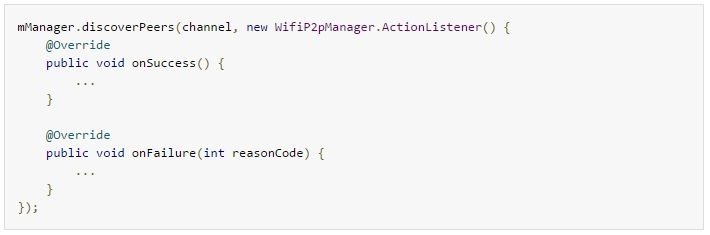
\includegraphics[width=1\textwidth]{imgs/discover_peers.jpg}
\captionof{figure}{Notifica di successo o fallimento per il metodo discoverPeers}\label{discover_peers_img}%
\end{center}

Se la fase di discoveri ha avuto successo e sono stati trovati nuovi Peers, il sistema di broadcast riceve un intento in WIFI P2P PEERS CHANGED ACTION, la lista dei peers si potrà ottenere tramite la chiamata del metodo requestPeers():

\begin{center}
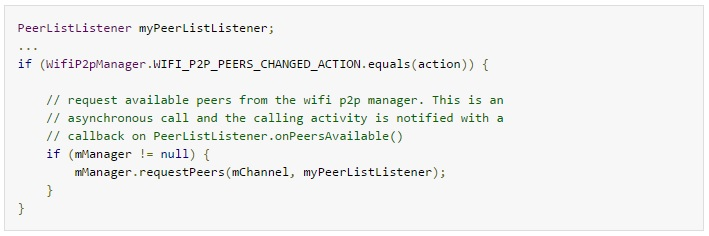
\includegraphics[width=1\textwidth]{imgs/intent_peers.jpg}
\captionof{figure}{Richiesta lista dei nuovi Peers}\label{intent_peers_img}%
\end{center}

Il metodo requestPeers() è anch'esso asincrono e può informare la nostra activity della presenza di una lista di nuovi Peers tramite il metodo onPeersAvailable() definito nell'interfaccia WifiP2pManager.PeerListListener.

\subsubsection{Connessione ai Peers}

Una volta trovato il dispositivo a cui vogliamo connetterci tra la lista dei Peers disponibili, sarà possibile connettersi ad esso tramite il metodo connect().
Tale metodo avrà bisogno di un oggetto WifiP2pConfig, all'interno del quale sono contenute le informazioni del dispositivo a cui vogliamo connetterci:

\begin{center}
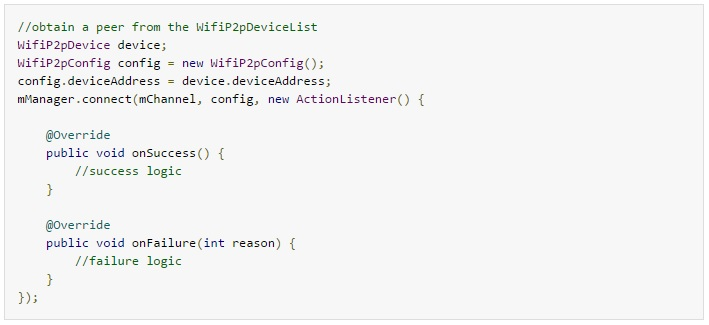
\includegraphics[width=1\textwidth]{imgs/connect.jpg}
\captionof{figure}{Metodo per permettere la connessione con un altro Peer}\label{connect_img}%
\end{center}

\subsubsection{Trasferimento Dati}

Una volta stabilita la connessione tra i due dispositivi, si può procedere con lo scambio di dati attraverso l'utilizzo di socket:

1- Creazione del ServerSocket, tale socket attenderà la connessione di un qualunque client sulla porta specificata e si bloccherà non appena l'avrà ricevuta (eseguire quindi questo processo all'interno di un thread).

2- Creazione di un ClientSocket, che userà indirizzo IP e porta definiti dal ServerSocket per connettersi ad esso.

3- Una volta che client e server saranno connessi si potrà procedere con lo scambio di dati tramite byte streams.

La figura \ref{server_img} illustrerà il codice impiegato lato Server per il trasferimento dei dati:


\begin{center}
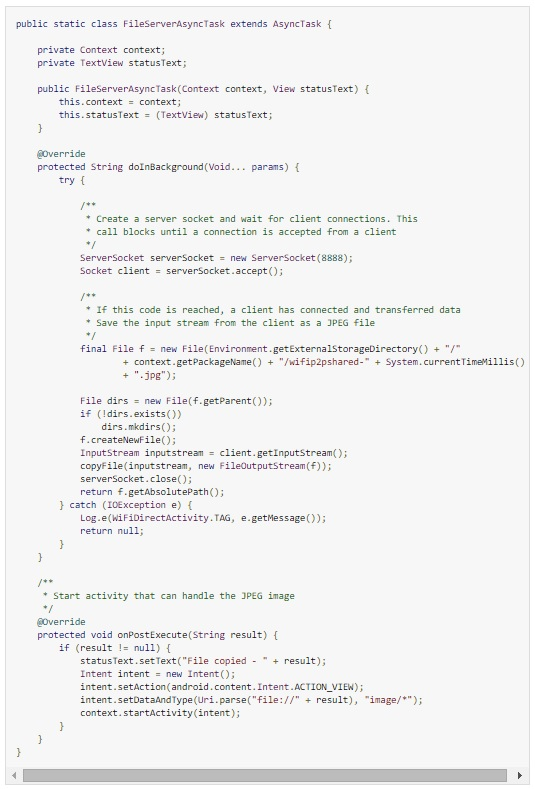
\includegraphics[width=1\textwidth]{imgs/server.jpg}
\captionof{figure}{Codice trasferimento dati lato Server}\label{server_img}%
\end{center}

La figura \ref{client_img} invece illustrerà la medesima cosa lato Client:

\begin{center}
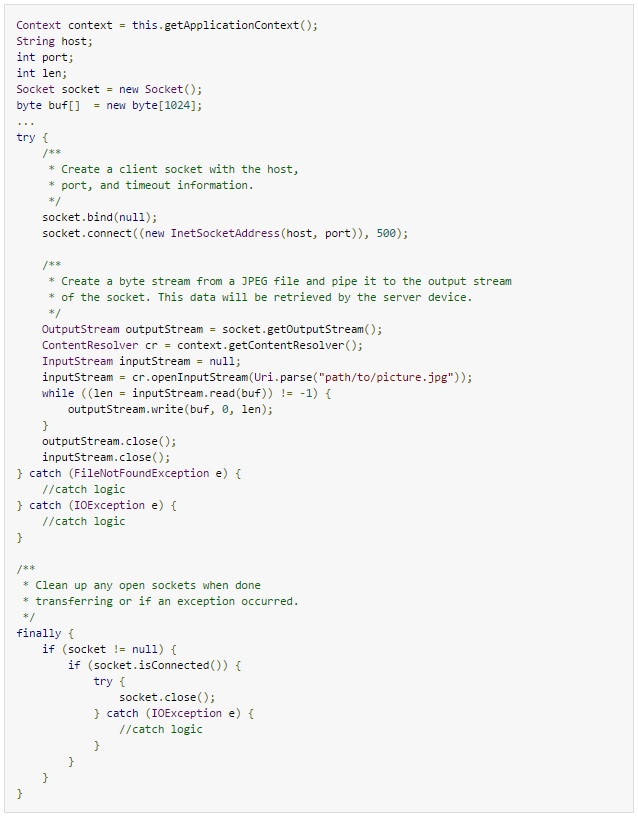
\includegraphics[width=1\textwidth]{imgs/client.jpg}
\captionof{figure}{Codice trasferimento dati lato Server}\label{client_img}%
\end{center}

\clearpage{\pagestyle{empty}\cleardoublepage}